\chapter{Theory}
\label{chap:theory}
\section{Arctic clouds}
The Arctic cloud cover is dominated by low clouds @cite. Most high amounts of stratus clouds are over the oceans~\citep{Klein1993}. The Arctic is the only region where the season of maximum stratus does not correspond to the season of greatest lower troposphere static stability~\citep{Klein1993}, which could be due to lack of evaporation during the cold winter months. According to~\cite{Klein1993} stratus in the Arctic basin peaks during summer at nearly 62\%, while during the winter season the stratus only accounts for 18\% of the cloud cover. This leads them to conclude that the seasonal cycle of stratus in the Arctic is driven by the temperature cycle, thereby moisture content in the atmosphere, rather than the static stability.(, as opposed to other areas.)

Are there any typical cloud properties special to the arctic? CURRY!

The air in the Arctic is very stable in winter (polar night) and clean as there are not many sources for pollution. In Autumn the sea ice extent reaches a minimum after the summer melting and leave open water to influence low clouds and their properties. 

Low clouds have bases below 2000 m. Stratus (St) are layered clouds that form when extensive areas of stable air are lifted. Stratus clouds are normally between 0.5 and 1~km thick, whereas they can be several km wide (@citeAguadoBurtpage188?).

\begin{figure}
\label{fig:dropletsize}
\centering
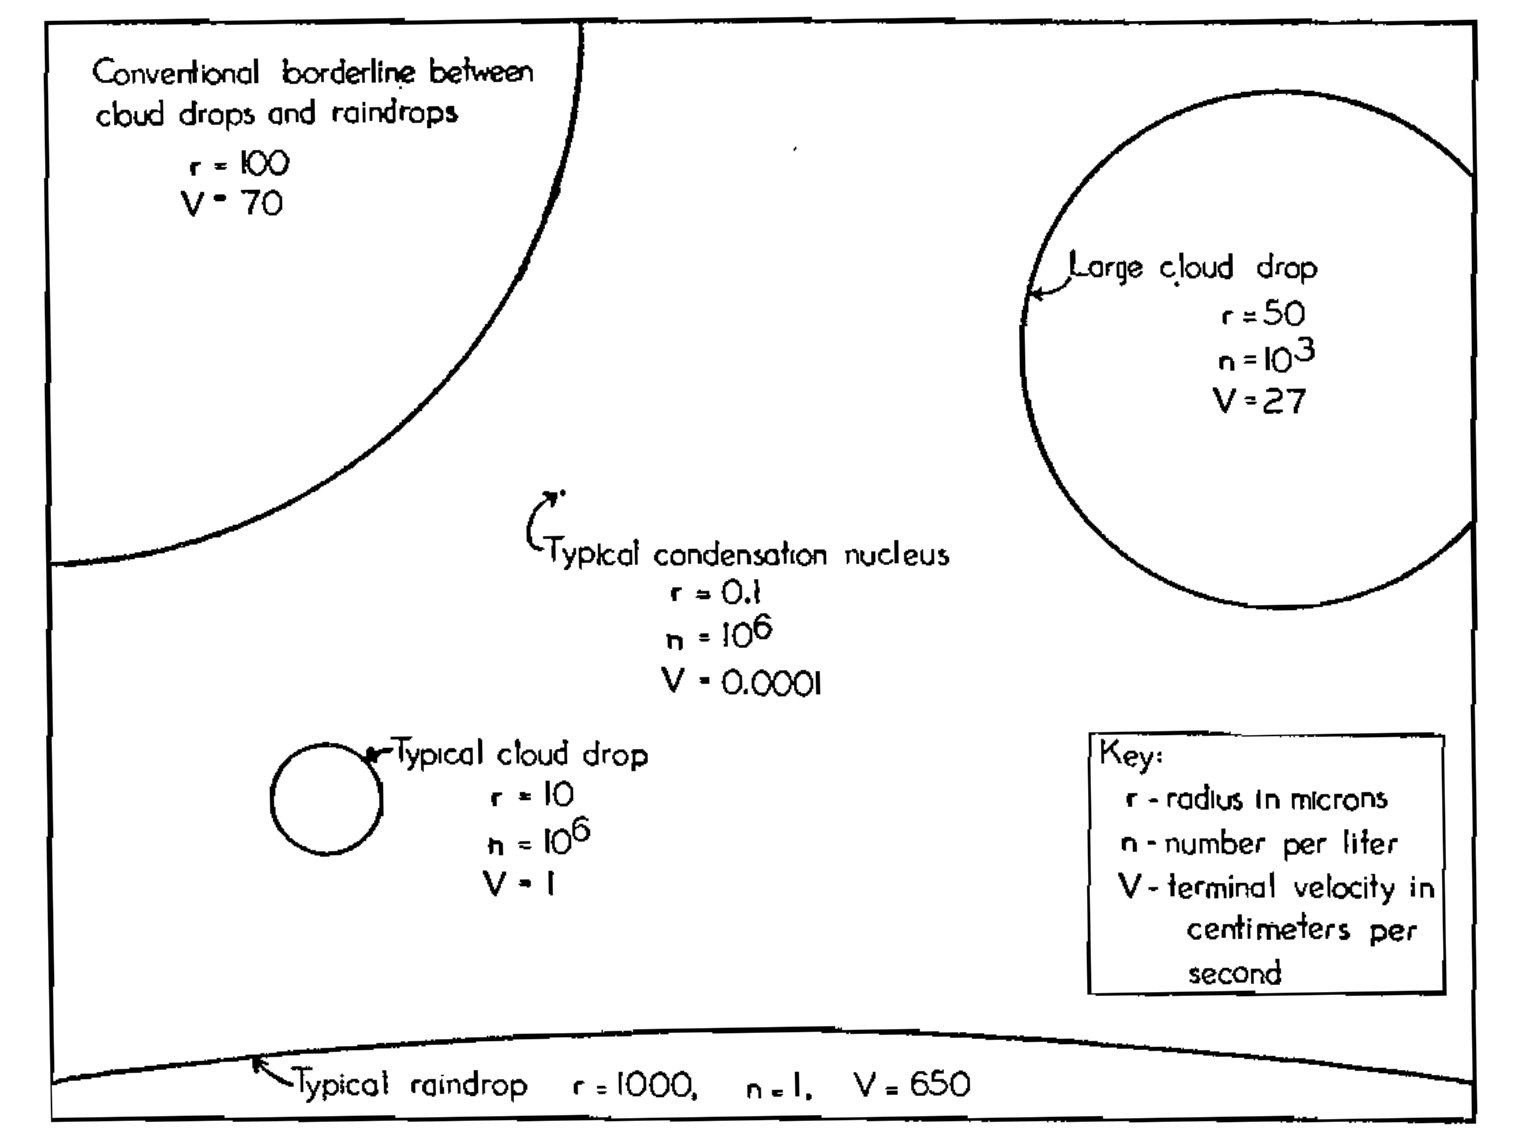
\includegraphics[width=1\textwidth]{dropletsize.png}
\caption{Size of CCN, typical cloud droplet, large cloud droplet, boarderline between cloud droplets and raindrops and typical size of raindrop. Adapted from~\citep{McDonald1958}.}
\label{fig:Schf01}
\end{figure}
 
\section{Radiation and clouds}
The cloud microphysical properties that determine the cloud radiative properties include: the amount of condensed water, the size and shape of the cloud particles, and the phase of the particles/and if the particles are liquid or ice~\citep{Curry1996}. The amount of condensed water can be expressed by the liquid water content (LWC) in the cloud, often presented with units $g~m^{-3}$, and is proportional to the median volume radius, $\overline{r}$, $\mju~m$. From~\cite{Rogers1989} we can express the number of droplets with radius $r$ by
\begin{equation}
N = \int n(r) dr
\end{equation}
where $N$ is the droplet number concentration $cm^{-3}$, and $n(r)$ is the number of droplets with radius $r$. @isit?
The LWC can be written
\begin{eqnarray}
LWC &=& \int \rho_L \frac{4}{3} \pi r^3 n(r) dr\\
&=& \frac{4}{3} \pi \rho_L \int r^3 n(r) dr\\
&=& \frac{4}{3} \pi \rho_L \overline{r}^3 \int n(r) dr\\
&=& \frac{4}{3} \pi \rho_L \overline{r}^3 N 
\end{eqnarray}
where the last equation shows the proportionality of LWC to the droplet number concentration $N$, and $\rho_L$ is the density of liquid water.

If the LWC is integrated over the height of the cloud, or any layer with chosen base and top in the atmosphere, we find the liquid water path (LWP) of that layer.
\begin{equation}
LWP = \int_{base}^{top} LWC dz
\end{equation}
The LWP is the column of liquid water in a cloud and is usually expressed by $g~m^{-2}$.


The cloud droplet effective radius determines many important radiative properties of a cloud and is therefore of particular interest. For example it determines the cloud albedo~\citep{Hansen1974}, which I will go more into when describing the first indirect effect.



Cloud consist of droplets that absorb, emit and scatter radiation. 
(introduction@)In this thesis shortwave (SW) radiation means solar radiation and longwave (LW) radiation covers the terrestrial infrared radiation.
How clouds scatter and absorb SW and LW radiation.
Explain something about blackbodies, clouds and blackbodies? Stefan–Boltzmanns law states that the flux density emitted by a blackbody is proportional to the fourth power of the absolute temperature @citeLiou2002page12. For a greybody, like a cloud, the equation can be written
\begin{equation}
F = \epsilon \sigma T^4
\end{equation}
where the emissivity of the greybody, $\epsilon$, is included. $F [W~m^{-2}]$ is the flux density emitted by the greybody, and $\sigma = 5.67\cdot 10^{-8} Jm^{-2}sec^{-1}deg^{-4}$ is the Stefan–Boltzmann constant.


Write about optical depth from Wallace and Hobbs: Normal optical depth or optical thickness, $\tau_{\lambda}$ is a measure of the cumulative depletion that a beam of radiation directed straight downward (zenith angle $\theta = 0$) would experience in passing through a defined layer \citep{WallaceHobbs2006}. The optical depth can be expressed as
\begin{equation}
\tau_{\lambda} = \int_z^{\infty} k_{\lambda} \rho r dz
\end{equation}
where $k_{\lambda}$ is the mass absorption coefficient, which has units of $m^2~kg^{-1}$, $\rho$ is the density of air, which has units of $kg~m^{-3}$, and $r$ is the mass of the absorbing gas per unit mass of air.



As mentioned in Chapter~\ref{chap:introduction} Introduction there is no solar radiation to reflect during winter and the polar night in the Arctic, where as in the summer the zenith angle is so high that even though there is sunlight 24 hours a day the cooling effect in summer does not average out the heating effect the clouds have in winter. The low clouds' ability to absorb and emit terrestrial radiation domiantes over their reflective effect on the solar radiation. @cite?

How do clouds reflect radiation? What is the effect of more water? Or more ice? What about the droplet size? (effective radius)\\
How do clouds absorb and emit radiation? Effect of more or less water or ice? Droplet size?

Ice is more effective in reflecting SW than water. Snow has a higher albedo than rain. Is there any use in presenting some albedo values for water, snow, ice? Or open water versus sea ice? New ice versus old sea ice?

Make sure to include something on how LWC/LWP and effective radii plays in, if this is to be mentioned in the results or discussion!!

\section{Aerosol effects on clouds}
Aerosols affect clouds in numerous ways. They have a direct effect on the climate by scattering and absorbing SW radiation. acting as CCNs og INs. elaborate?
Diminishing sea ice could lead to an increase in the aerosol number concentrations in the area where ice has retreated. The open sea surface it self would lead to an increase in release of sea salt to the lower atmosphere @cite. The lack of sea ice would also increase the likelyhood that the sea could be used for shipping, which would pollute the area @cite. There are two known indirect effects that aerosols have on radiation, through clouds. The first indirect effect was proposed by~\cite{Twomey1974} and is some times referred to as the Twomey effect. The second indirect effect was proposed by~\cite{Albrecht1989} @citecorrectly 

\subsection{The first indirect effect} (Maybe just call it all indirect effects and refer to Lohmann and Feichter)
The first indirect effect, suggested by~\cite{Twomey1974}, describes the enhancement of cloud albedo as a consequence of an increase in aerosol content and thereby available CCNs.
In short, the first indirect effect is a cloud albedo enhancement.
By increasing droplet concentration and hence the optical thickness of a cloud, pollution acts to increase the reflectance of clouds~\citep{Twomey1977}. 
The optical thickness is increased when the number of CCN is increased. Although the changes are small, the long term effects on climate can be profound~\citep{Twomey1974}.

Meg: The optical depth will change with changes in aerosol number concentrations and changes in clouds and their properties. For instance if a cloud has many small droplets, the optical depth will be higher. Where as  fewer cloud droplets will yield a lower optical depth, resulting in more SW radiation reaching the ground — possibly having a warming effect on the area. 


\subsection{The second indirect effect}
Albrecht 1989 
The second indirect effect, or the cloud lifetime effect, suggests more numerous but smaller droplets reduce the precipitation efficiency and by that enhances the cloud lifetime and hence the cloud reflectivity~\citep{Albrecht1989}. This effect has been estimated to be of roughly as large as the first indirect effect~\citep{Lohmann2005}.


Production of DMS by phytoplankton Charlson 1987


